% Copyright (C) 2023 by Kağan ÖZGÜN
% E-mail: ozgunk@itu.edu.tr

\documentclass{article}
\usepackage[T1]{fontenc}
\usepackage[utf8]{inputenc}
\usepackage{changes}
\definechangesauthor[name=proposal, color=red]{pp}
\usepackage{booktabs}% A package to produce nice looking tables
\usepackage{graphicx}% A package to include graphics
\usepackage{algorithm}
\usepackage{algpseudocode}
\usepackage{algorithmicx}

\algdef{SE}[VARIABLES]{Variables}{EndVariables}
   {\algorithmicvariables}
   {\algorithmicend\ \algorithmicvariables}
\algnewcommand{\algorithmicvariables}{\textbf{input variables}}


\author{Kağan Özgün}
\title{Predicting Denial of Service Attacks Using Network Traffic Dataset}

\begin{document}
\maketitle

\begin{abstract}
-
\end{abstract}

\section{Introduction}
Shortly after the emergence of personal computers, people began to encounter the definitions of cyber attack and cyber attacker. The methods used by these malicious people who want to damage computers or access data on these devices have changed over time with the advancement of technology. Due to the fact that the internet was not widespread in the beginning, malicious software spread over input and output devices was used a lot. With the increase in the use of the
Internet, the attackers started to make their attacks mainly over the network. With the spread of systems such as antivirus or intrusion detection systems (IDS) used to prevent this situation,
attackers began to look for methods that could be launched more insidiously. Denial of service (DoS) attacks, which became widespread in the early 2000s \cite{Rangapur}, has also been
one of the attack types that emerged for this purpose. DoS attacks generally aim to temporarily or long-term takedown of a targeted resource. In order to increase the effect of these attacks, similar attacks made from many points are called distributed denial of service attacks(DDoS). 

DDoS attacks are also divided into various categories according to the types of packets and requests they use, the frequency change of the number of requests used, and their purposes. In the prevention of these attack types, devices called IDS are used, which mainly include rule-based analysis and send network packets to the devices that provide service after passing this analysis. Since rule-based devices are insufficient in emerging attack types, it is preferred to use machine learning-based methods that can learn from incoming data.

Detecting file attacks instantly or detecting incoming attack types is very important for detecting future attacks and learning attack types. For this purpose, many different classification studies have been carried out in the literature and very successful results have been obtained in both binary and multi-class classification processes, especially in DL-based studies. What is more important than the instant detection of the incoming attack type by classification is to determine that the attack will start a certain time before the attack comes. Predicting an attack can give network security experts a huge advantage in preventing an attack.

Within the scope of this study, it is aimed to predict DoS attacks that will occur for a certain period by using a Long Short-Term Memory(LSTM) based model. Model training and evaluation phases include two different commonly used public network datasets. Used techniques and approaches are detailed in the following section and the result of the proposed solution and reference are model compared in the evaluation section. 

\subsection{Problem definition}
DoS attacks, which attack methods aimed at restricting the accessibility of applications or directly preventing the application from being accessible, are one of the greatest dangers, especially for applications with many users and sessions. In particular, during campaign times or if the application infrastructure is already under load, long-term problems may occur in the application exposed to such attacks. It may take time for the systems to be accessible again. Accessibility is a significant factor in areas such as banking, insurance and e-commerce, and the reliability of the application is severely damaged if it is under DoS attack.

\subsection{Motivation}
Although various studies have been carried out on detecting and preventing DoS attacks, it is still one of the most common attack types today. DoS attacks, first encountered and defined in 1999, became more widespread after the 2010s, and the severity of the attacks increased over the years\cite{Rangapur}. For handling the increase in DoS attacks more successful and flexible attack detection systems developed and different approaches proposed. In recent years the usage of artificial intelligence-based methods increased for this reason and they generate better predictions for attack detection. It gives very successful results in estimation, especially due to the memory structure used by LSTM-based models. For this reason, predicting DoS attacks with LSTM-based models can produce good results. This study, it is aimed to predict DoS attacks with an LSTM-based model before the attack occurs and to ensure that cyber security experts or systems take the necessary precautions.

\subsection{Solution hypothesis}

In the study, 3 different models were tried with two different datasets, and it was aimed to achieve at least one of these models over 75\% accuracy in both datasets. In addition, it is desired to observe how the LSTM-based model will perform compared to other models.

\subsection{Contribution}

The results of these experiments were observed by making an experiment to predict D0S attacks, which are not very common in the literature before the attack occurs. In this way, it has been tried to show how possible it is to predict DoS attacks. In addition, the performance of a deep learning(DL) based model has been observed against the traditional rule-based approach and the widely used Gaussian Naive Bayes(GNB) method. In this way, it is discussed how competent DL-based models can be in this field, and it is aimed to put forward different research questions on such models and predicting DoS attacks.

\section{Methodology}

In this section, there is detailed information about the datasets used in the study, how these datasets are processed and the models developed. In the experimental phase of the study, two cyber attack datasets derived from different structures and three different models were used.

\subsection{Dataset Selection}

Since the purpose of this study is to detect DoS attacks, which is one of the common attack types in computer networks, we needed network data for model development and experimentation phases. First of all, we aimed to work on a dataset obtained from a real system, but since network data contains valuable information such as personal information and IP address, port of companies' systems, companies do not volunteer to share this data. For this reason, we searched for datasets used in similar studies. In accordance with the purpose of our study, we found two different datasets through similar studies. The first of these datasets is a derived cyber-attack dataset released under the name UNSW-NB15. The second dataset was the CIC-DDoS2019, which was specifically derived from DoS attacks and included different types of DoS attacks. Since these two datasets are derived, we preferred to have at least two different datasets in our study. 

\subsubsection{UNSWNB-15}

UNSW-NB15 is a dataset created by the Cyber Range Lab at the University of New South Wales(UNSW) \cite{Unswnb15}. This dataset has been prepared using the IXIA PerfectStorm tool to cover normal activities and synthetic attacks in modern networks. The network data in the established simulation environment has been recorded as raw network data with the tcpdump tool and contains 100GB of data in total. The Dataset includes nine different attack types which are Fuzzers, Analysis, Backdoors, DoS, Exploits, Generic, Reconnaissance, Shellcode and Worms; apart from normal traffic data. This data, which was derived using The Argus and Bro-IDS tools, was processed to become a dataset containing 49 different features and a label column. The data set containing 49 columns was shared as csv files with a total of 2,540,044 rows.

\subsubsection{CIC-DDoS2019}

The CICDDoS2019 dataset, created by researchers at the Canadian Institute for Cybersecurity (CIC), University of New Brunswick (UNB), is data produced specifically for research on DDoS) attacks \cite{CICDDoS2019}. While creating this data set, modern attack types and normal network data are used. While creating the simulation environment, the network data generated by 25 different users using HTTP, HTTPS, FTP, SSH and email protocols are derived. Different operating systems and versions were also used in the simulation environment. Since it is aimed to simulate subtypes of DDoS attacks, data belonging to 13 different DDoS attack types known as NTP, DNS, LDAP, MSSQL, NetBIOS, SNMP, SSDP, UDP, UDP-Lag, WebDDoS, SYN, TFTP and SYN were produced. This dataset, collected as raw data, contains 87 features and 70,619,331 rows of data. While the dataset was shared, a data set containing the best 14 features was also shared with it.

\subsection{Data Preparation}

Since the purpose of this study is to predict DDoS attacks before they happen, we need to bring the historical data into a certain format. For this reason, some operations were performed on both datasets. Various similar operations were performed for the rule-based, LSTM-based and Naive Bayes model used in this study. Basically, the purpose of DoS attacks is to attack by using the IP and port information of the target determined from different devices. For this reason, training and testing sets were prepared by applying grouping operations in the dataset. Source IP addresses, destination IP addresses and destination port information of packets in the network are used in grouping processes. Different approaches have been applied for each model and these processes are explained in detail in the following section. While grouping, source ip destination port information and destination IP address and destination port information were used in the UNSW-NB15 dataset. However, when the same grouping was made in the CIC-DDoS2019 dataset, due to the structure of the dataset, sufficient data groups could not be created when binary groupings were made. For this reason, groupings in the CIC-DDoS2019 dataset were made using target IP information and source IP information.

We applied a simple grouping process to prepare the datasets for the prediction process. In order to do the prediction, we had to use the source IP-Port and destination IP-Port information that we have and obtained from the incoming network data, since the main purpose of danial of service attacks is to send intensive packets from certain sources to certain destinations. In this way, we have predicted whether there will be an attack from the source of a packet arriving at time t. Thanks to this system, people responsible for network security will be offered the opportunity to block packets from certain sources. Since DoS attacks are not made from a single source in general, we wanted to predict whether a packet from any source would attack after t time instead of making all data to be used for forecasting have the same source or destination information while grouping the data. In order to use the datasets we have effectively in the testing phase, we chose the source and destination information of a packet arriving at time t and the packets at the distance we want to make predictions to be the same while making this grouping. If these models are used in real systems, there will be no need to do this in the prediction phase. 

\subsubsection{Rule-Based Model}

In the rule-based model, the main purpose is to mark the incoming packets as attacks when they exceed a certain limit by keeping the number of packets coming from similar sources and going to similar destinations. Since there is no training process in the rule-based model, train test validation splits are not created in this model. All data was processed and marking was done on the incoming data. The actual labels of the network packets were used to determine the success of this model. In the grouping stage, 20, 50, 100 and 200 packages were brought together and it was tried to estimate 300, 600, 1200, 1800, 2400 and 3000 packages from the last package in the combined data. While choosing the distances of the target packets to the packets used in the rule, the time elapsed between the packets in the dataset was taken as a basis. Since on average 10 milliseconds passed between each packet, it was tried to estimate approximately 30 seconds, 1 minute, 2 minutes, 3 minutes, 4 minutes and 5 minutes by using target distances.

\begin{figure}
  \centering
  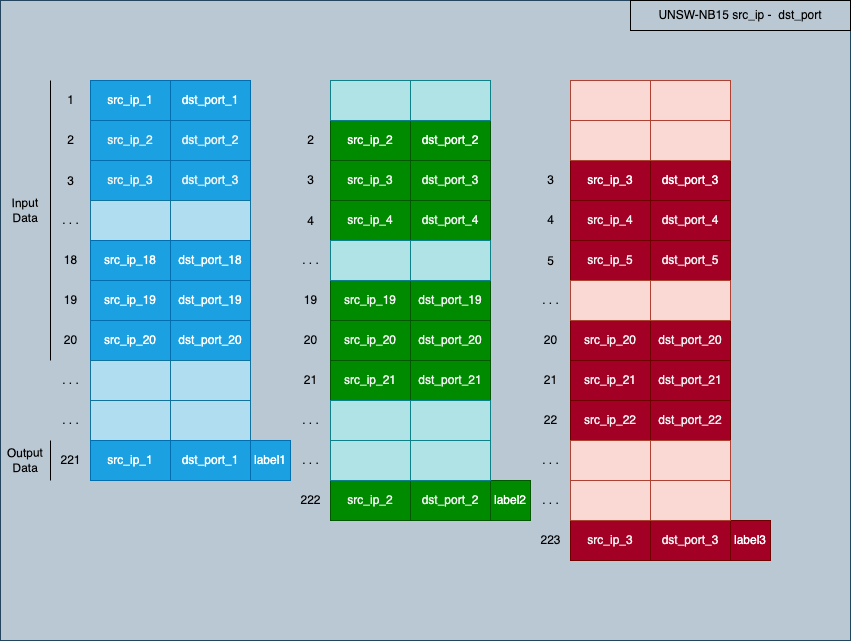
\includegraphics[width=\textwidth]{unswnb15_rule_based.png}
  \caption{UNSW-NB15 (Source IP - Destination Port) Rule Based Data Preparation}
  \label{unswnb15-rule-based}
\end{figure}

Source IP destination port and destination IP destination port pairs are used in UNSW-NB15 dataset. The generated dataset is visualized in figure ~\ref{unswnb15-rule-based}.

\begin{figure}
  \centering
  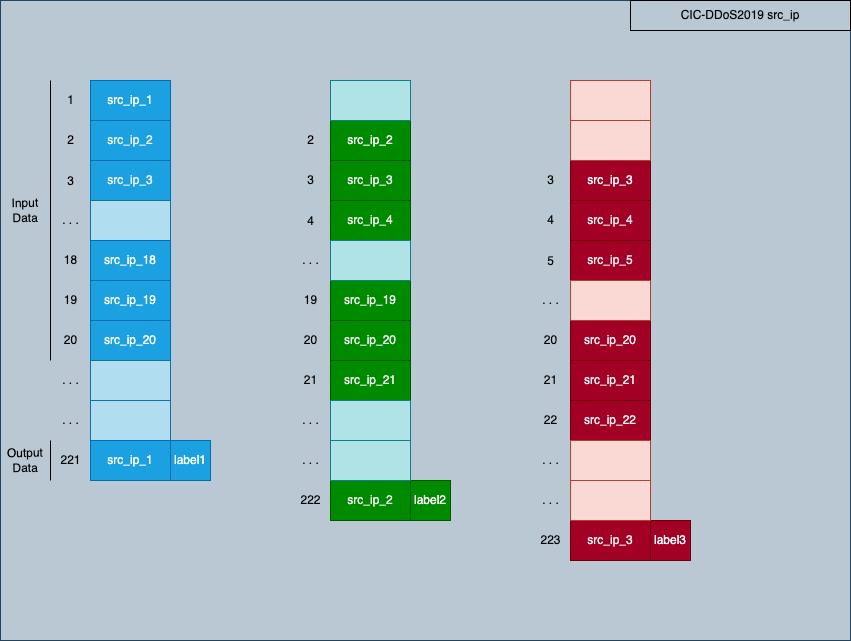
\includegraphics[width=\textwidth]{cicddos2019_rule_based.png}
  \caption{CICDDoS2019 (Source IP) Rule Based Data Preparation}
  \label{cicddos2019-rule-based}
\end{figure}

Grouping depends on to source IP or destination IP approach used in the CICDDoS2019 dataset. The generated dataset is visualized in figure ~\ref{cicddos2019-rule-based}.
 

\subsubsection{Gaussian Naive Bayes Model}

Gaussian Naive Bayes is a widely used simple method that uses the distribution of data to classify, but it is a method that can produce effective results. For this reason, we used it as one of the base models in this direction in the project. In the study, we used the 'Gaussian Naive Bayes' model available in the 'sklearn' library. Due to the structure of this model, we only needed train and test datasets, so we separated train test separation as 70\% train and 30\% test. In the dataset we have, we take a certain number of sequential network data and use it to classify the future network packet at a certain distance from the dataset. For this reason, we used a large number of previous network packets for each classification operation. However, due to its structure, the 'Gaussian Naive Bayes' model in the 'sklearn' library can only work with two-dimensional datasets. In order to make the datasets we have suitable for this model, we added the relevant columns of the data packets to be processed as input to the model and turned them into a single row containing many columns, and made the classification of the future packet at a distance determined with this data. The dataset was created by selecting the best 10 features selected in each dataset. For each predicting process, 20, 50,100 and 200 network data were used and to see the effect of the forecasting process at different distances, predictions were made for the next 300, 600, 1200, 1800, 2400 and 3000 packets from the last packet in the datasets used. As in the rule-based model, different grouping operations were applied in UNSW-NB15 and CICDDoS2019 datasets. Chart of these stages are shared in figure ~\ref{unswnb15-gnb} and figure ~\ref{cicddos2019-gnb} as examples for each dataset.

\begin{figure}
  \centering
  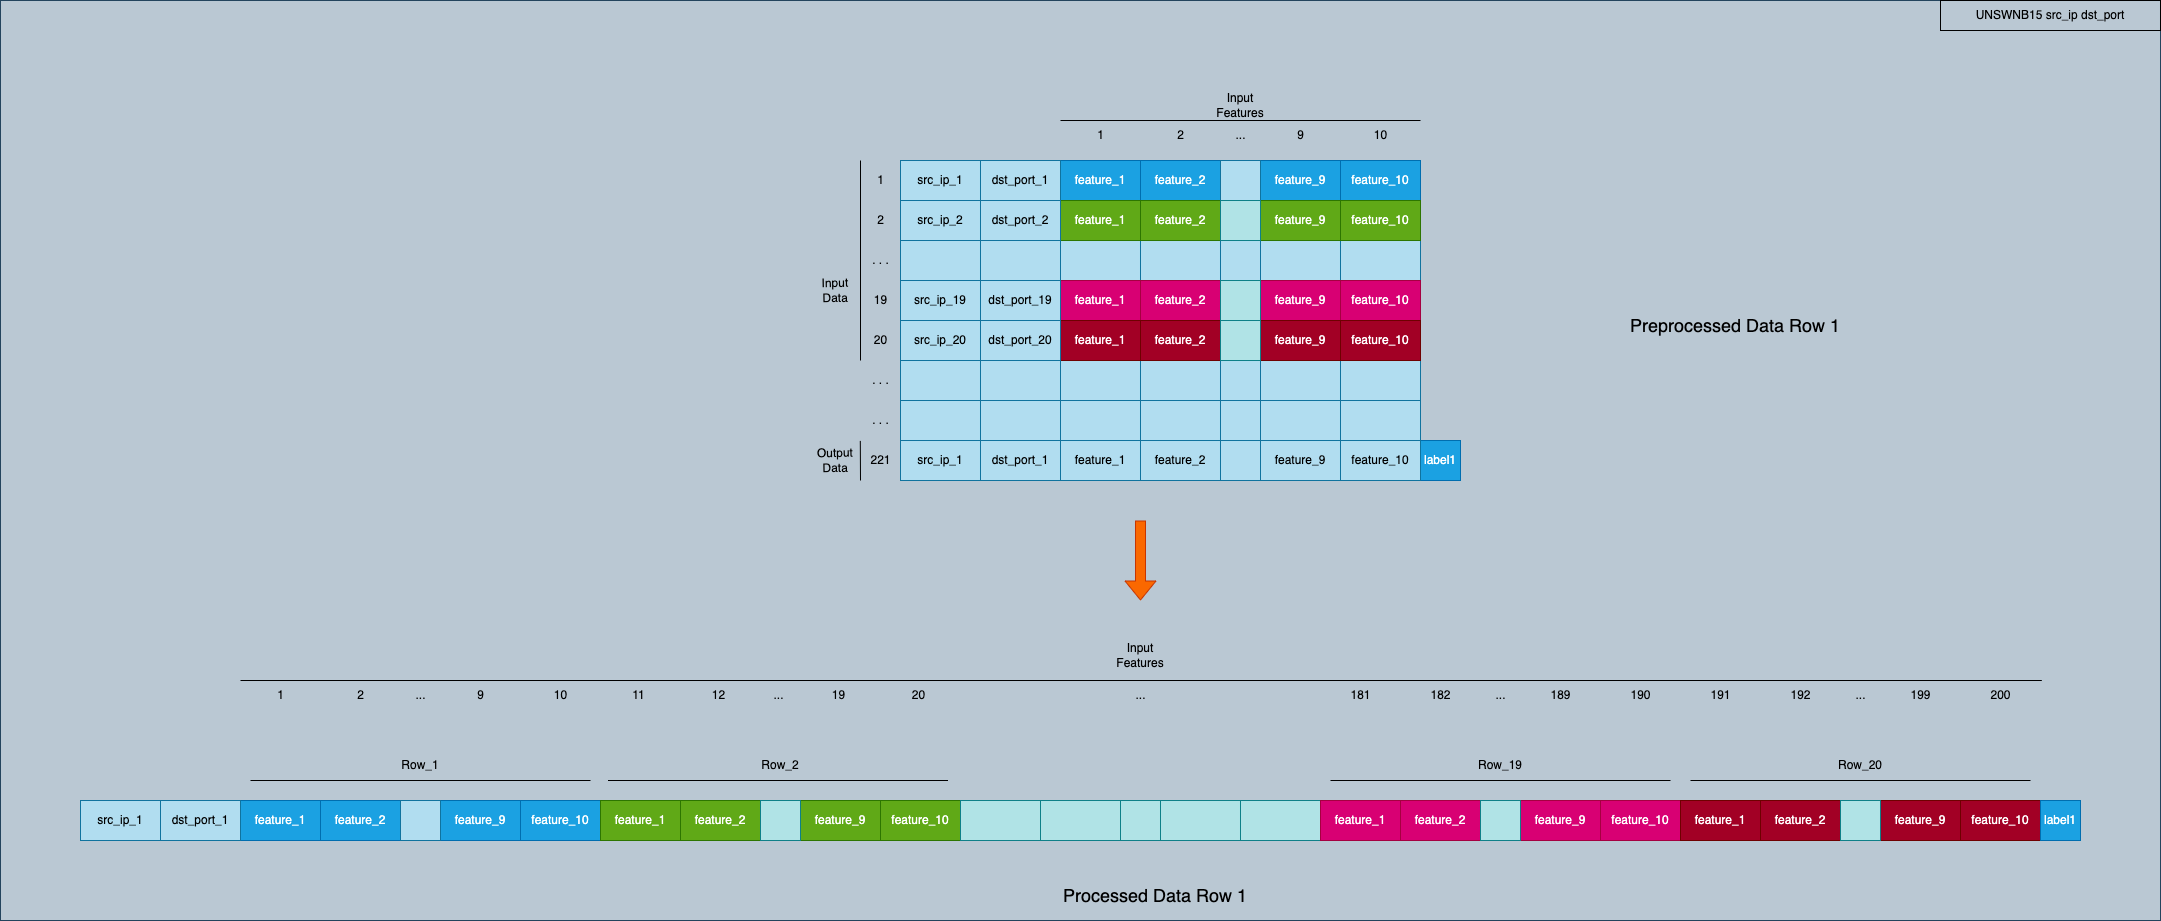
\includegraphics[width=\textwidth]{unswnb15_gnb.png}
  \caption{UNSW-NB15 (Source IP - Destination Port) Gaussian Naive Bayes Data Preparation}
  \label{unswnb15-gnb}
\end{figure}

\begin{figure}
  \centering
  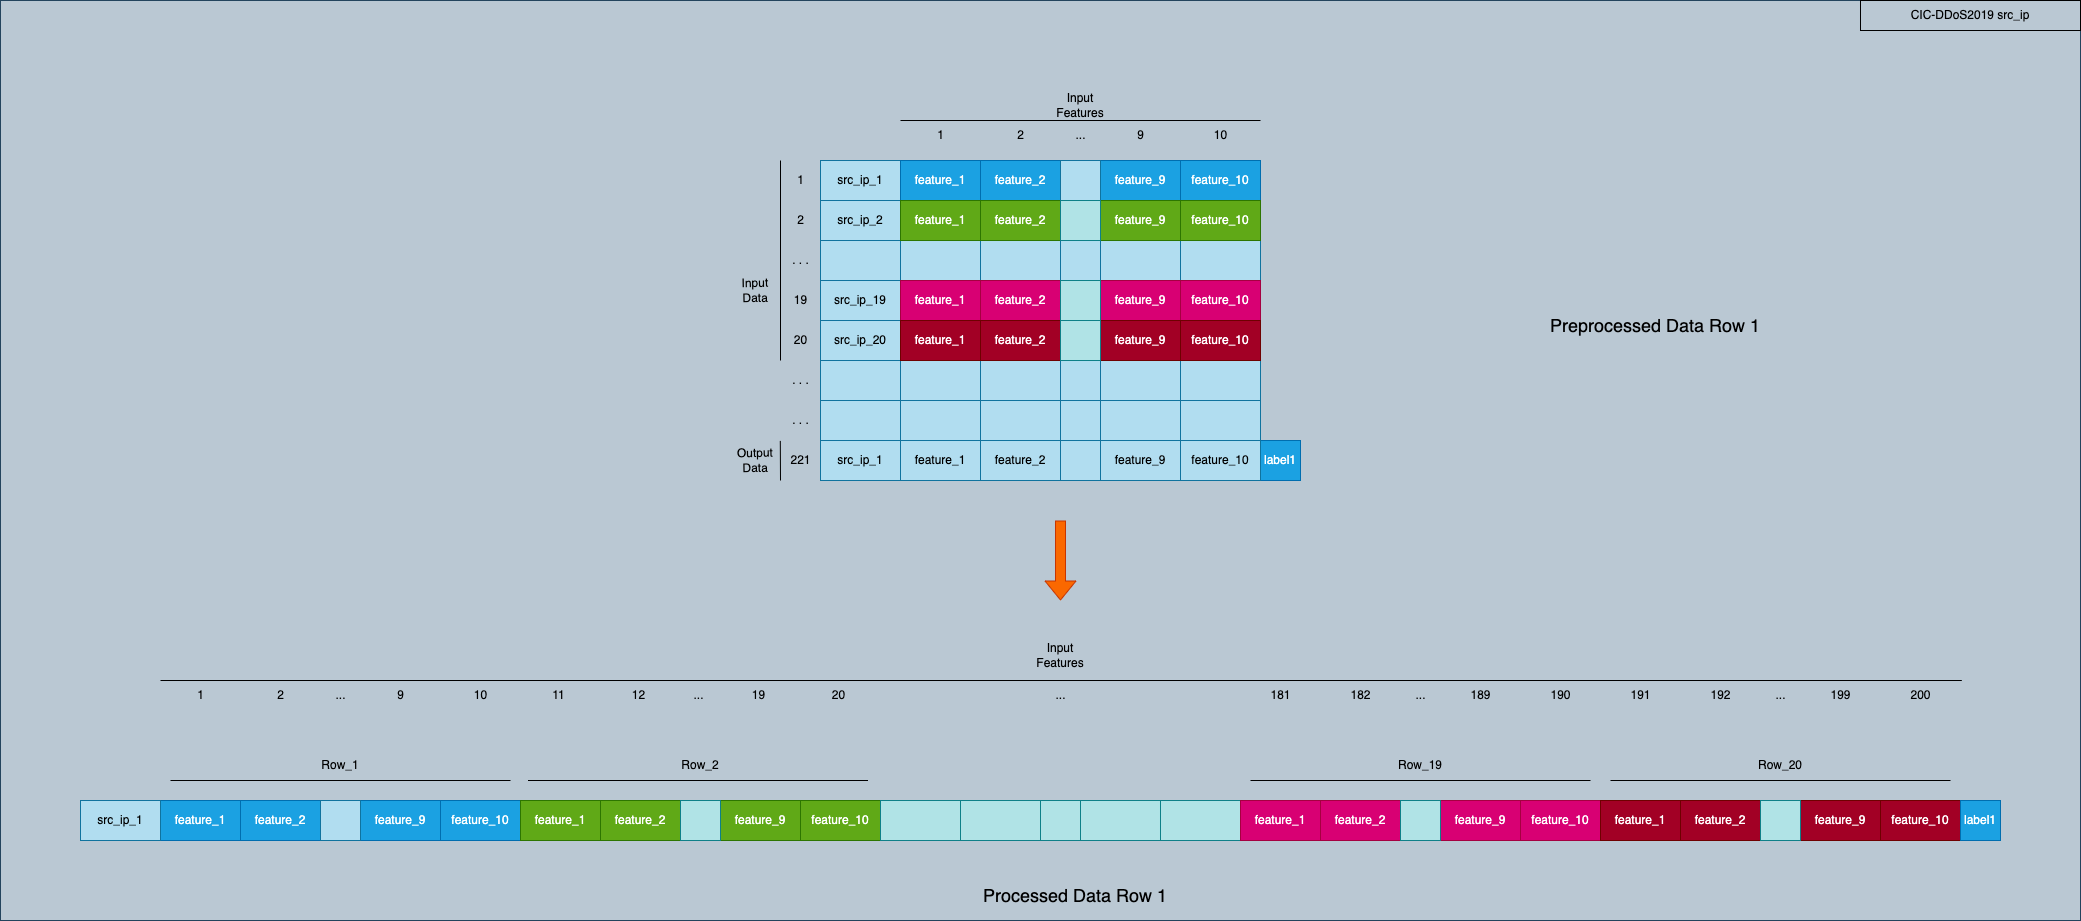
\includegraphics[width=\textwidth]{cicddos2019_gnb.png}
  \caption{CICDDoS2019 (Source IP) Gaussian Naive Bayes Data Preparation}
  \label{cicddos2019-gnb}
\end{figure}

\subsubsection{Long Short-Term Memory(LSTM) Model}

Some of the operations we used while preparing the GNB data for the data set used for the LSTM model were used in common. Since the LSTM model has the capacity to process three-dimensional data, the process of adding each row side by side, which was applied in GNB, was not applied in this model. As in GNB, the datasets were created to make predictions for a certain number of pre-forecasting data and future data at a specified distance from these data. Differently, the model was run using different train, test and validation splits, so that the model was not overfitted and we had the opportunity to compare the results obtained with data at different rates. Different data split processes were applied as 70\% train 30\% test, 60\% train 20\% validation 20\% test and 60\% train 10\% validation 20\% test data. The datasets obtained as a result of the data processing operations for the LSTM model are shown in figure ~\ref{unswnb15-lstm} and figure ~\ref{cicddos2019-gnb}.

\begin{figure}
  \centering
  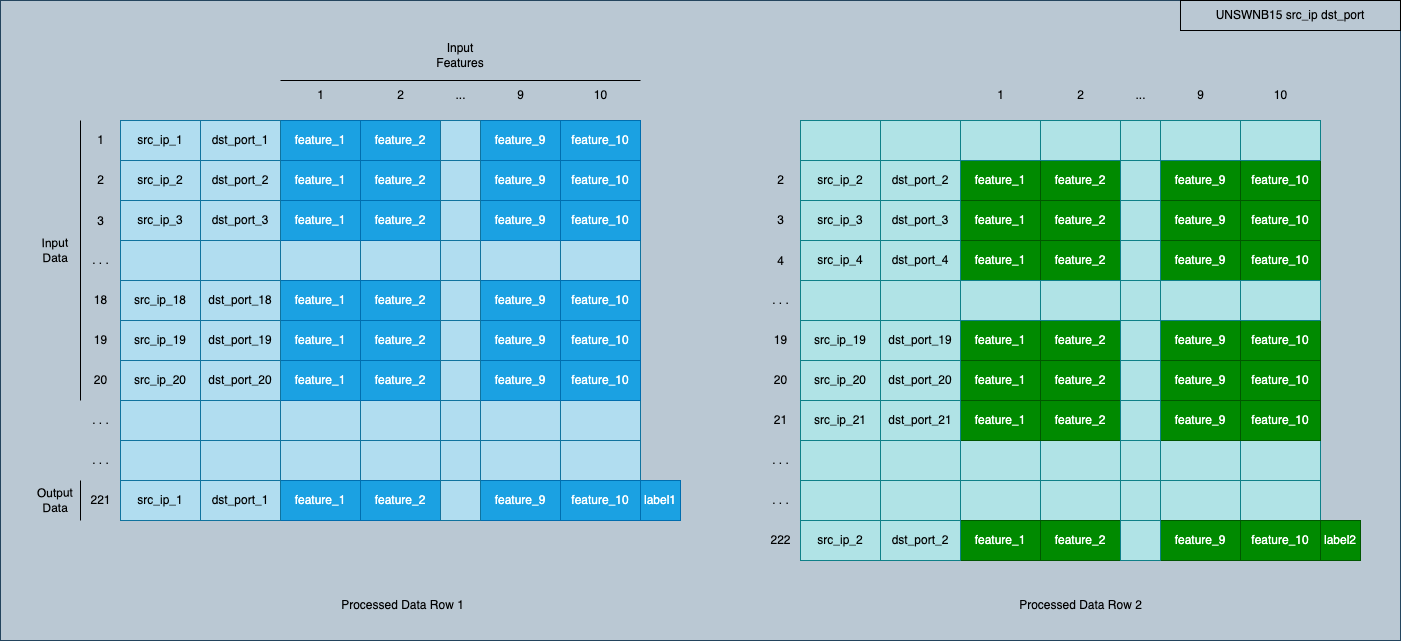
\includegraphics[width=\textwidth]{unswnb15_lstm.png}
  \caption{UNSW-NB15 (Source IP - Destination Port) LSTM Data Preparation}
  \label{unswnb15-lstm}
\end{figure}

\begin{figure}
  \centering
  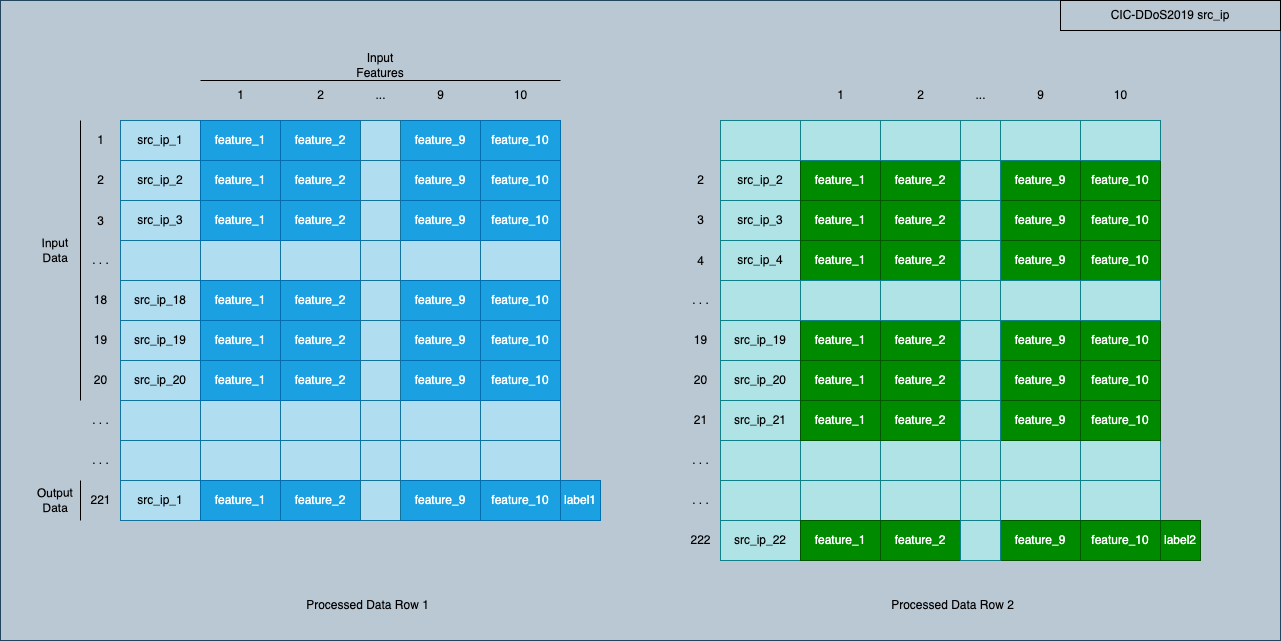
\includegraphics[width=\textwidth]{cicddos2019_lstm.png}
  \caption{CICDDoS2019 (Source IP) LSTM Data Preparation}
  \label{cicddos2019-lstm}
\end{figure}

\subsection{Model Development}
Details about model that developed in this work given in the sub section. Data preparation and model development phase of the project published in public git repository ~\cite{ozgunk}.

\subsubsection{Rule-Based Model}

The rule-based model is included in this study because it is a simple model that is frequently used in non-AI-based approaches and is familiar to network security experts. Another reason for adding the rule-based model is to observe how effective a prediction is made using only the source and destination information of incoming packets. 

The rule-based model is a method that evaluates whether the incoming network packets have certain source and destination pairs with very simple data processing operations. In this approach, it is necessary to set certain limits for the information of whether there will be an attack according to the incoming packets. Normally, setting these limits by people who have been observing the network traffic for a long time can lead to good results. But this is risky as it is a fairly open approach to human error. In addition, it is a method that will escape the attention of experts and cause problems when changing attack types or methods used for the first time. 

The rule-based approach created within the scope of the study was tried to be estimated over the number of packets containing the same source and destination information in the datasets grouped according to the source IP - destination port or destination IP destination-port information for the UNSW-NB15 dataset. In the CICDDoS2019 dataset, the groupings were made according to the source IP or destination IP information and the rule was operated according to this information. As a limit, 1, 2, 3, 4 and 5 were tested during the experiment. For example, if the limit is selected as 1, if the dataset used as input has more than one packet containing the same target and source information, such packets are marked as attacks. 

If the limit is 1, the model will tend to flag a large number of packets as attacks, or if the limit is selected larger, it will tend to select most of the packets as normal. Accordingly, there will be deviations in false negative and false positive values of this approach. While testing this approach, the amount of input was chosen differently as 20, 50, 100 and 200 packages. At this point, although the limits are chosen similarly, an ideal rule-based algorithm should also consider the amount of input. The effects of this situation were observed in the experiments. The estimation periods were selected as 300, 600, 1200, 1800, 2400 and 3000 post-packages in all models, so that estimations were made for approximately 30 seconds to 300 seconds later.

\subsubsection{Gaussian Naive Bayes Model}

Examining the distribution of data, which is one of the main rules and is frequently used in basic statistics and data science, can be sufficient to produce good results for many problems. Using similar approaches for intrusion detection in computer networks can provide simple but effective models. For this reason, the GNB model, which can perform classification using the Gaussian distribution, was used as the base model in our study. This model can very simply learn the distribution in the training dataset and test whether the test dataset is suitable for this distribution and label the test data.

This simple but effective model has one drawback, which is that it requires the input dataset to fit the distribution in order to get a good model. This model, which can produce effective results in a dataset containing known attack types and network movements, may fail in a dataset that comes for the first time or that has different distributions. The efficacy of this model is directly affected by the dataset's suitability for distribution and the frequency of change. For this reason, we can call this model a simple effective model that cannot easily adapt to changing conditions.

Within the scope of our study, we used the GNB model in the Python sklearn library. For the training and testing phase of this model, we have divided our dataset as 70\% train and 30\% test. We did not use other train-test splits for the rule-based model as this model does not use validation sets. The procedures applied to make the datasets suitable for this model are explained in detail in the data preparation section.

\subsubsection{Long Short-Term Memory(LSTM) Model}

The main purpose of this study is to predict DoS attacks before they happen, using sequential network patterns in the time-series format. For this estimation process, we thought that there was a need to develop a model that can work with different datasets and is more flexible than previous models and can learn from data. We have developed a model that includes the LSTM structure, which is very powerful and effective especially on time-series data.

LSTM layers are one of the structures that can process historical data and adapt to changing data, thanks to the different memory types it contains in the DL approach. For this reason, we chose to build a two-layer LSTM model that is not very complex in the structure we created. We wanted to observe the results we obtained on different data types by comparing the results we obtained thanks to the created model with the GNB and rule-based approach.

The LSTM model we created basically includes two different LSTM layers. While the first of these layers consists of 32 units, we preferred to use an LSTM structure containing 16 units in the second layer. We prevented the model from being overfit by adding the Dropout layer between these two layers. In the last layer of our model, we added the Dense layer, which includes the sigmoid activation function, as our aim is to make binary classfication. The general structure of our model is shown in figure ~\ref{lstm-model}.

\begin{figure}
  \centering
  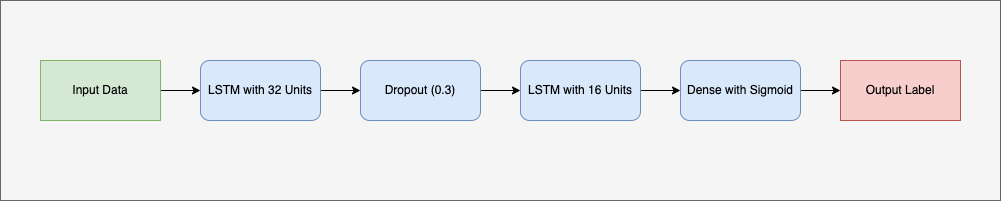
\includegraphics[width=\textwidth]{lstm_model.png}
  \caption{LSTM Model Structure}
  \label{lstm-model}
\end{figure}

The data set used in the LSTM model was run with the same amount of input input options and the same estimation windows as the previous models. In addition, training and testing stages of the model were implemented using different train, test and validation splits. In these different trials, 60\% train 20\% validation 20\% test, 60\% train 10\% validation 20\% test and 70\% train 30\% test splits were used.

\section{Related work}

TODO


A study on designing a system that detects especially HTTP flood and TCP flood type DoS attacks by examining tags and flags in network data with statistical methods has been done by Shaaban et al\cite{Shaaban}. As a result of this study, a model that is said to detect DoS attack types for 3 seconds after the start of the attack is proposed, but no metrics for the performance of this model are given. Method used in this project includes more complex DL algorithms comparing to Shaaban et al's work. Additionally, evaluation result are detailed and performance evaluation metrics like accuracy, false negative rates and recall used in proposed method evaluation section. Also, a reference model results added to evaluation process.

In another study, Sitiawan and other researchers aimed to detect Ping Flood attacks, a kind of DoS attack, using IoT network data with the K-Means method \cite{Stiawan}. 
In this study, both accuracy value and confusion matrix results are shared as performance metrics, and a successful result was revealed according to these results. However, the dataset used in the study contains approximately 95\% of attack data and 5\% of normal data, which is different from real-life scenarios. For this reason, the realistic performance of this approach will be different from the experiment. Our methodology includes three different dataset and each of the dataset processed before model development phase for simulating real world scenarios.

In their study, which was published in 2022, Gopi et al. developed a model on DoS attack detection with an ANN-based DL model\cite{Gopi}. In this study, it is desired to present a successful model that can predict faster than a standard Artificial Neural Network (ANN) model using dimension reduction approaches. However, similar to the previous study dataset used includes more attack data than normal network traffic. Dataset used in this publication has 30\% of normal traffic and 70\% of attack traffic. In the result section of the paper proposed model performance is compared with an ANN model. Comparing to this work, our methodology has different kind of DL models and a reference model for generate realistic evaluation. Besides, balanced datasets that includes 70\% of normal traffic and 30\% of attack traffic used in proposed methodology.

In another study by Yan Li and Yifei Lu, a model that detects DoS attacks was developed using a model that includes LSTM and Bayes methods. A comparison was made with the model containing only LSTM in the conclusion part\cite{Li}. In the conclusion part of this study, a sample study, the result of a base model and the result of the proposed model are compared, and the results are given with different metrics. However, as in other studies, the dataset used was chosen in a balanced way, containing 50\% normal 50\% attack traffic, unlike the network traffic encountered under normal conditions. In Yan Li and Yifei Lu's study DL models hat include LSTM layer used similar to our proposed model and in evaluation section different evaluation criteria and detailed results provided in paper. However, different kind of dataset are not used in their work. Working with single dataset decrease the reliability of the results and proposed method in realistic environment. For increasing reliability of the proposed method and results three different dataset used in our proposed work.

Developing a DL-based model for detecting DoS attacks includes complex neural network structures and complex calculations. Some of the researchers proposed a DL model with complex feature extraction and feature manipulation methods to increase the efficiency of the models. Luhan Zou and other contributors proposed a model with a feature grouping technique\cite{LuhanZou}. This approach is named feature-attended multi-flow long short-term memory (FAMF-LSTM) by the authors. The technique includes a future engineering part with grouping input features depending on similarities then they feed different groups to a LSTM-based model for predicting DoS attacks in the dataset. They used BoT-IoT and UNSW-NB15 datasets for the training and test phase of the work.
Results show their proposed hypothesis is correct. The proposed model got better accuracy compared to models without feature manipulations. However, fine-optimized DL-based models can get better results without feature manipulation. In some specific cases, feature manipulation can generate better results but for DoS detection using BoT-IoT and UNSW-NB15 datasets, additional feature operation is not needed. Optimized RNN or LSTM models can achieve better results compared to the method proposed by Luhan Zout et. al.

Detecting the attacks depends on network data structure and attack-normal traffic rate in the dataset. In the real-world scenario, most of the network traffic is generated by normal users so it includes normal traffic heavily. However, generated datasets generally include more attack traffic compared to normal traffic of the network. This situation cause difference between the success of the model on the test dataset and the real-world scenario. Due to solve that problem, using dataset balancing techniques can be reasonable. Jirasin Boonchai and other researchers used the data balancing method for handling this problem. They used the Synthetic Minority Oversampling Technique (SMOTE) technique for solving the imbalance issue of the CIC-DDoS2019 dataset\cite{Jirasin}. Dataset samples were created using SMOTE for each class label and the new sampled dataset includes 50\% of attack and 50\% of normal traffic. After sampling they trained DNN-based and convolutional autoencoder-based models and compare the result of the models with  Naive Bayes and Logistic Regression models. Proposed models got better predictions compared to reference models but accuracy and other metrics are not good enough compared to solutions in the literature. For solving the imbalance problem, a similar approach is used in our work but SMOTE is not used. A sampling method depends on python numpy library used for generating balanced sampled datasets. 30\% attack traffic and 70\% normal traffic ratio are preferred in the proposed method in this work because this ratio is more realistic compared to 50-50 ratio.   

Brief comparison of the related work and proposed methodology provided in Table~\ref{comtable}. Comparison table includes three specific information about related works and proposed method. 

\begin{table}
  \centering
  \caption{Comparison of the related work methodology
  }
  \label{comtable}
  \begin{tabular}{lrrr}
    \toprule
	~ & \multicolumn{1}{p{2cm}}{\centering Include \\ DL Model} & \multicolumn{1}{p{2cm}}{\centering Multiple \\ Dataset} & \multicolumn{1}{p{2cm}}{\centering Multiple \\ Evaluation \\ Criteria}\\
	\midrule
    Proposed Solution & \textbf{YES} & \textbf{YES} & \textbf{YES}    \\
	\cite{Shaaban}    & NO           & NO          & NO \\
	\cite{Stiawan}    & NO           & YES           & YES \\
	\cite{Gopi}       & YES          & NO           & YES  \\
	\cite{Li}         & YES           & NO           & YES \\
	\cite{LuhanZou}   & \textbf{YES} & \textbf{YES} & \textbf{YES}    \\
	\cite{Jirasin}   & YES           & NO           & YES \\
	\bottomrule
  \end{tabular}
\end{table}

\section{Results}

Within the scope of the study, the results of two different datasets and three different models were brought together in this section and the results were compared.

\subsection{Results of UNSW-NB15}

The important results of the experiments with the UNSW-NB15 dataset were brought together in this section and information about the results of the experiment was shared.

\subsubsection{Rule-Based Model}

In the experiments conducted using the rule-based model, two different groups were made on the UNSW-NB15 dataset during the data processing phase. The best results and the worst results obtained for each grouping operation are combined in this section. In this way, the performance of the model under different configurations was examined.

The best result for 'Destination IP - Destination Port' grouping was obtained when we gave 20 input data to this model and estimated for 300 packets, and these results are shown in Table ~\ref{unswnb15-rule-based-dst-ip-dst-port-best}. Also, worst result for 'Destination IP - Destination Port' grouping was obtained when we gave 200 input data to this model and estimated for 3000 packets, and these results are shown in Table ~\ref{unswnb15-rule-based-dst-ip-dst-port-worst}.

When we analyzed the results, the rule-based approach was not successful in the UNSW-NB15 dataset, which mainly contains normal traffic packets. Although this approach did not give very bad results in detecting the packets containing attacks in this dataset, its overall performance decreased as it contained too many false negative and false positive values in the overall result. 

When we look at the best and worst results obtained, it has been observed that there is not much difference between them, and all experiments with this dataset have achieved a success rate of 55\%.

\begin{table}
  \centering
  \caption{UNSW-NB15 Rule Based Model Destination IP - Destination Port Best Result}
  \label{unswnb15-rule-based-dst-ip-dst-port-best}
  \begin{tabular}{lrrrrrrr}
    \toprule
	{Rule & Accuracy & Recall 0 & Recall 1 & Precision 0 & Precision 1 & F1 Score 0 & F1 Score 1} \\
	\midrule
        >1 & 0,5091 & 0,0233 & 0,9989 & 0,9559 & 0,5036 & 0,0454 & 0,6696 \\ \hline
        >2 & 0,5236 & 0,0531 & 0,9979 & 0,9617 & 0,5111 & 0,1006 & 0,6759 \\ \hline
        >3 & 0,5384 & 0,0842 & 0,9964 & 0,9598 & 0,5190 & 0,1547 & 0,6826 \\ \hline
        >4 & 0,5512 & 0,1111 & 0,9948 & 0,9559 & 0,5261 & 0,1991 & 0,6882 \\ \hline
        \textbf{>5} & \textbf{0,5621} & \textbf{0,1348} & \textbf{0,9930} & \textbf{0,9508} & \textbf{0,5323} & \textbf{0,2361} & \textbf{0,6931} \\
	\bottomrule
  \end{tabular}
\end{table}

\begin{table}
  \centering
  \caption{UNSW-NB15 Rule Based Model Destination IP - Destination Worst Result}
  \label{unswnb15-rule-based-dst-ip-dst-port-worst}
  \begin{tabular}{lrrrrrrr}
    \toprule
	{Rule & Accuracy & Recall 0 & Recall 1 & Precision 0 & Precision 1 & F1 Score 0 & F1 Score 1} \\
	\midrule
        >1 & 0,4977 & 0,0235 & 0,9984 & 0,9381 & 0,4919 & 0,0458 & 0,6591 \\ \hline
        >2 & 0,5126 & 0,0537 & 0,9970 & 0,9501 & 0,4995 & 0,1017 & 0,6655 \\ \hline
        >3 & 0,5289 & 0,0869 & 0,9955 & 0,9536 & 0,5080 & 0,1593 & 0,6727 \\ \hline
        >4 & 0,5428 & 0,1158 & 0,9937 & 0,9513 & 0,5156 & 0,2065 & 0,6789 \\ \hline
        \textbf{>5} & \textbf{0,5541} & \textbf{0,1393} & \textbf{0,9920} & \textbf{0,9485} & \textbf{0,5219} & \textbf{0,2429} & \textbf{0,6840} \\ 
	\bottomrule
  \end{tabular}
\end{table}

The best result for the 'Source IP - Destination Port' grouping was obtained when we gave 50 input data to this model and estimated 2400 packets, and these results are shown in Table ~\ref{unswnb15-rule-based-src-ip-dst-port-best}. Also, the worst result for the 'Source IP - Destination Port' grouping was obtained when we gave 200 input data to this model and estimated 300 packets, and these results are shown in Table ~\ref{unswnb15-rule-based-src-ip-dst-port-worst}.

When we analyzed the results, the rule-based approach was not successful in the UNSW-NB15 dataset, which mainly contains normal traffic packets. Although this approach did not give very bad results in detecting the packets containing attacks in this dataset, its overall performance decreased as it contained too many false negative and false positive values in the overall result.

When we examine the results we obtained for this type of grouping, it was observed that although we obtained similar results with the other grouping method in the best configuration, the performance fell below 50\% in the experiment that produced the worst result.

\begin{table}
  \centering
  \caption{UNSW-NB15 Rule Based Model Source IP - Destination Port Best Result}
  \label{unswnb15-rule-based-src-ip-dst-port-best}
  \begin{tabular}{lrrrrrrr}
    \toprule
	{Rule & Accuracy & Recall 0 & Recall 1 & Precision 0 & Precision 1 & F1 Score 0 & F1 Score 1} \\
	\midrule
        \textbf{>1} & \textbf{0,5531} & \textbf{0,5525} & \textbf{0,5538} & \textbf{0,5584} & \textbf{0,5478} & \textbf{0,5554} & \textbf{0,5508} \\ \hline
        >2 & 0,5520 & 0,5674 & 0,5362 & 0,5555 & 0,5482 & 0,5614 & 0,5421 \\ \hline
        >3 & 0,5505 & 0,5846 & 0,5156 & 0,5522 & 0,5486 & 0,5679 & 0,5316 \\ \hline
        >4 & 0,5492 & 0,6023 & 0,4950 & 0,5492 & 0,5492 & 0,5745 & 0,5207 \\ \hline
        >5 & 0,5484 & 0,6209 & 0,4743 & 0,5468 & 0,5505 & 0,5815 & 0,5096 \\
	\bottomrule
  \end{tabular}
\end{table}

\begin{table}
  \centering
  \caption{UNSW-NB15 Rule Based Model Source IP - Destination Port Worst Result}
  \label{unswnb15-rule-based-src-ip-dst-port-worst}
  \begin{tabular}{lrrrrrrr}
    \toprule
	{Rule & Accuracy & Recall 0 & Recall 1 & Precision 0 & Precision 1 & F1 Score 0 & F1 Score 1} \\
	\midrule
        >1 & 0,4793 & 0,1926 & 0,7667 & 0,4528 & 0,4865 & 0,2703 & 0,5952 \\ \hline
        >2 & 0,4793 & 0,1928 & 0,7665 & 0,4529 & 0,4865 & 0,2705 & 0,5952 \\ \hline
        >3 & 0,4793 & 0,1930 & 0,7664 & 0,4529 & 0,4865 & 0,2706 & 0,5952 \\ \hline
        >4 & 0,4793 & 0,1931 & 0,7661 & 0,4529 & 0,4865 & 0,2708 & 0,5951 \\ \hline
        >5 & 0,4792 & 0,1932 & 0,7659 & 0,4528 & 0,4864 & 0,2709 & 0,5950 \\ 
	\bottomrule
  \end{tabular}
\end{table}

\subsubsection{Gaussian Naive Bayes Model}

As in the rule-based model, two different groupings were made on the data in the GNB-based model. From our experiments with the 'Destination IP - Destination Port' grid, we got the best result when we fed 50 packets as input. The details of the results are shown in Table ~\ref{unswnb15-gnb-dst-ip-dst-port-best}. When we observed the results, we observed that it was a very successful model. A very successful estimation was made in all of the different metrics we used.

The worst results obtained in our experiments are also shared in Table ~\ref{unswnb15-gnb-dst-ip-dst-port-worst} and this result obtained when we feed 20 network package to model. When we look at these results, we can say that it produces very bad results compared to the results we get with the best configuration. The negative value of false is too high because this model, which successfully predicts normal network traffic, fails to predict attack packets.

\begin{table}
  \centering
  \caption{UNSW-NB15 GNB Model Destination IP - Destination Port Best Result}
  \label{unswnb15-gnb-dst-ip-dst-port-best}
  \begin{tabular}{lrrrrrrr}
    \toprule
	{ Pred Win & Accuracy & Recall 0 & Recall 1 & Precision 0 & Precision 1 & F1 Score 0 & F1 Score 1} \\
	\midrule
        300 & 0,9405 & 0,9970 & 0,8845 & 0,8954 & 0,9967 & 0,9435 & 0,9373 \\ \hline
        600 & 0,9574 & 0,9982 & 0,9174 & 0,9221 & 0,9981 & 0,9587 & 0,9561 \\ \hline
        1200 & 0,9869 & 0,9986 & 0,9751 & 0,9760 & 0,9985 & 0,9872 & 0,9867 \\ \hline
        1800 & 0,9877 & 0,9987 & 0,9765 & 0,9775 & 0,9986 & 0,9880 & 0,9874 \\ \hline
        2400 & 0,9954 & 0,9988 & 0,9919 & 0,9922 & 0,9988 & 0,9955 & 0,9953 \\ \hline
        \textbf{3000} & \textbf{0,9981} & \textbf{0,9992} & \textbf{0,9970} & \textbf{0,9971} & \textbf{0,9992} & \textbf{0,9982} & \textbf{0,9981} \\ 
	\bottomrule
  \end{tabular}
\end{table}

\begin{table}
  \centering
  \caption{UNSW-NB15 GNB Model Destination IP - Destination Port Worst Result}
  \label{unswnb15-gnb-dst-ip-dst-port-worst}
  \begin{tabular}{lrrrrrrrrr}
    \toprule
	{ Pred Win & Accuracy & Recall 0 & Recall 1 & Precision 0 & Precision 1 & F1 Score 0 & F1 Score 1} \\
	\midrule
        300 & 0,5469 & 0,9999 & 0,0021 & 0,5465 & 0,9500 & 0,7067 & 0,0042 \\ \hline
        600 & 0,5480 & 0,9988 & 0,0030 & 0,5478 & 0,6667 & 0,7075 & 0,0059 \\ \hline
        1200 & 0,5533 & 0,9998 & 0,0020 & 0,5529 & 0,8947 & 0,7121 & 0,0040 \\ \hline
        1800 & 0,5501 & 0,9990 & 0,0023 & 0,5500 & 0,6441 & 0,7094 & 0,0045 \\ \hline
        2400 & 0,5504 & 0,9997 & 0,0025 & 0,5500 & 0,8750 & 0,7096 & 0,0050 \\ \hline
        3000 & 0,5567 & 0,9991 & 0,0032 & 0,5564 & 0,7286 & 0,7147 & 0,0063 \\ 
	\bottomrule
  \end{tabular}
\end{table}

From our experiments with the 'Source IP - Destination Port' grid, we got the best result when we fed 50 packets as input. The details of the results are shown in Table ~\ref{unswnb15-gnb-src-ip-dst-port-best}. When we observed the results, we observed that it was a very successful model. A very successful estimation was made in all of the different metrics we used.

The worst results obtained in our experiments are also shared in Table ~\ref{unswnb15-gnb-src-ip-dst-port-worst}. When we look at these results, we can say that it produces very bad results compared to the results we get with the best configuration. The negative value of false is too high because this model, which successfully predicts normal network traffic, fails to predict attack packets.

\begin{table}
  \centering
  \caption{UNSW-NB15 GNB Model Source IP - Destination Port Best Result}
  \label{unswnb15-gnb-src-ip-dst-port-best}
  \begin{tabular}{lrrrrrrrrr}
    \toprule
	{ Pred Win & Accuracy & Recall 0 & Recall 1 & Precision 0 & Precision 1 & F1 Score 0 & F1 Score 1} \\
	\midrule
        300 & 0,9388 & 0,9969 & 0,8812 & 0,8926 & 0,9965 & 0,9419 & 0,9353 \\ \hline
        600 & 0,9517 & 0,9983 & 0,9052 & 0,9132 & 0,9981 & 0,9538 & 0,9494 \\ \hline
        1200 & 0,9805 & 0,9987 & 0,9617 & 0,9642 & 0,9986 & 0,9811 & 0,9798 \\ \hline
        1800 & 0,9812 & 0,9988 & 0,9634 & 0,9650 & 0,9988 & 0,9816 & 0,9808 \\ \hline
        2400 & 0,9898 & 0,9992 & 0,9801 & 0,9811 & 0,9992 & 0,9901 & 0,9895 \\ \hline
        \textbf{3000} & \textbf{0,9974} & \textbf{0,9992} & \textbf{0,9956} & \textbf{0,9957} & \textbf{0,9992} & \textbf{0,9975} & \textbf{0,9974} \\ 
	\bottomrule
  \end{tabular}
\end{table}

\begin{table}
  \centering
  \caption{UNSW-NB15 GNB Model Source IP - Destination Port Worst Result}
  \label{unswnb15-gnb-src-ip-dst-port-worst}
  \begin{tabular}{lrrrrrrrrr}
    \toprule
	{ Pred Win & Accuracy & Recall 0 & Recall 1 & Precision 0 & Precision 1 & F1 Score 0 & F1 Score 1} \\
	\midrule
        300 & 0,5455 & 1,0000 & 0,0021 & 0,5451 & 1,0000 & 0,7056 & 0,0041 \\ \hline
        600 & 0,5482 & 0,9991 & 0,0030 & 0,5479 & 0,7260 & 0,7077 & 0,0060 \\ \hline
        1200 & 0,5521 & 0,9999 & 0,0020 & 0,5517 & 0,9444 & 0,7111 & 0,0039 \\ \hline
        1800 & 0,5513 & 0,9991 & 0,0023 & 0,5512 & 0,6667 & 0,7104 & 0,0045 \\ \hline
        2400 & 0,5503 & 0,9997 & 0,0025 & 0,5499 & 0,8571 & 0,7095 & 0,0050 \\ \hline
        3000 & 0,5563 & 0,9991 & 0,0030 & 0,5559 & 0,7273 & 0,7144 & 0,0059 \\ 
	\bottomrule
  \end{tabular}
\end{table}

\subsubsection{Long Short-Term Memory(LSTM) Model}

TODO: Tables will updated after end of all experiments

The results of the experiments performed with the 'Destination IP - Destination Port' pair in the experiments performed with the LSTM model are shown in Table ~\ref{unswnb15-lstm-dst-ip-dst-port-best}. When we examine these results, we can say that my performance is lower than GNB, but we have achieved success between 70\% - 80\% in all metrics.

The results of the experiments performed with the 'Source IP - Destination Port' pair in the experiments performed with the LSTM model are shown in Table ~\ref{unswnb15-lstm-src-ip-dst-port-best}. When we examine these results, we can say that my performance is lower than GNB, but we have achieved success between 70\% - 80\% in all metrics. When we examined these results, we realized that my performance was slightly lower when compared to the previous grouping approach.


\begin{table}
  \centering
  \caption{UNSW-NB15 LSTM Model Destination IP - Destination Port Result}
  \label{unswnb15-lstm-dst-ip-dst-port-best}
  \begin{tabular}{lrrrrrrr}
    \toprule
	{Pred Win & Accuracy & Recall 0 & Recall 1 & Precision 0 & Precision 1 & F1 Score 0 & F1 Score 1} \\
	\midrule
        300 & 0,7628 & 0,7593 & 0,7673 & 0,8044 & 0,7166 & 0,7812 & 0,7411 \\ \hline
        600 & 0,7780 & 0,8295 & 0,7138 & 0,7833 & 0,7705 & 0,8057 & 0,7411 \\ \hline
        1200 & 0,7560 & 0,7294 & 0,7900 & 0,8161 & 0,6955 & 0,7703 & 0,7397 \\ \hline
        1800 & 0,7745 & 0,8265 & 0,7100 & 0,7795 & 0,7674 & 0,8023 & 0,7376 \\ \hline
        2400 & 0,7798 & 0,8192 & 0,7303 & 0,7921 & 0,7630 & 0,8054 & 0,7463 \\ \hline
        3000 & 0,7895 & 0,8279 & 0,7398 & 0,8044 & 0,7688 & 0,8160 & 0,7540 \\
	\bottomrule
  \end{tabular}
\end{table}

\begin{table}
  \centering
  \caption{UNSW-NB15 LSTM Model Source IP - Destination Port Result}
  \label{unswnb15-lstm-src-ip-dst-port-best}
  \begin{tabular}{lrrrrrrr}
    \toprule
	{Pred Win & Accuracy & Recall 0 & Recall 1 & Precision 0 & Precision 1 & F1 Score 0 & F1 Score 1} \\
	\midrule
        300 & 0,7821 & 0,8159 & 0,7397 & 0,7973 & 0,7621 & 0,8065 & 0,7507 \\ \hline
        600 & 0,7517 & 0,7400 & 0,7664 & 0,7986 & 0,7020 & 0,7682 & 0,7328 \\ \hline
        1200 & 0,7661 & 0,7687 & 0,7628 & 0,8047 & 0,7217 & 0,7863 & 0,7417 \\ \hline
        1800 & 0,7657 & 0,7697 & 0,7607 & 0,8005 & 0,7258 & 0,7848 & 0,7428 \\ \hline
        2400 & 0,7780 & 0,8030 & 0,7467 & 0,7995 & 0,7509 & 0,8012 & 0,7488 \\ \hline
        3000 & 0,7514 & 0,7191 & 0,7930 & 0,8170 & 0,6871 & 0,7650 & 0,7362 \\ 
	\bottomrule
  \end{tabular}
\end{table}

\subsection{Results of CIC-DDoS2019}

The important results of the experiments with the CICDDoS2019 dataset were brought together in this section and information about the results of the experiment was shared.

\subsubsection{Rule-Based Model}

In the experiments conducted using the rule-based model, two different groups were made on the CICDDoS2019 dataset during the data processing phase. The best results and the worst results obtained for each grouping operation are combined in this section. In this way, the performance of the model under different configurations was examined.

The best result for the 'Destination IP' grouping was obtained when we gave 20 input data to this model and estimated 300 packets, and these results are shown in Table ~\ref{cicddos2019-rule-based-dst-ip-best}. Also, the worst result for the 'Destination IP' grouping was obtained when we gave 200 input data to this model and estimated 3000 packets, and these results are shown in Table ~\ref{cicddos2019-rule-based-dst-ip-worst}.

When we analyzed the results, the rule-based approach was very successful in the CICDDoS2019 dataset, which mainly contains attack traffic packets. This situation is caused by the limited values we give to the rule-based approach. Since the values we give are very small compared to the number of packets, an approach has emerged that considers most packets as attacks, and this may result in a large number of false positive predictions. The overall performance seems to be successful since the attack data is dense in our data.

When we look at the best and worst results obtained, it has been observed that there is not much difference between them, and all experiments with this dataset have achieved a success rate of above 97\%.

\begin{table}
  \centering
  \caption{CICDDoS2019 Rule Based Model Destination IP Best Result}
  \label{cicddos2019-rule-based-dst-ip-best}
  \begin{tabular}{lrrrrrrr}
    \toprule
	{Rule & Accuracy & Recall 0 & Recall 1 & Precision 0 & Precision 1 & F1 Score 0 & F1 Score 1} \\
	\midrule
        >1 & 0,9593 & 0,0533 & 0,9997 & 0,8879 & 0,9595 & 0,1006 & 0,9792 \\ \hline
        >2 & 0,9614 & 0,1087 & 0,9994 & 0,8886 & 0,9618 & 0,1938 & 0,9802 \\ \hline
        >3 & 0,9635 & 0,1665 & 0,9991 & 0,8893 & 0,9641 & 0,2804 & 0,9813 \\ \hline
        >4 & 0,9659 & 0,2288 & 0,9988 & 0,8923 & 0,9667 & 0,3642 & 0,9825 \\ \hline
        \textbf{>5} & \textbf{0,9684} & \textbf{0,2931} & \textbf{0,9985} & \textbf{0,8946} & \textbf{0,9694} & \textbf{0,4415} & \textbf{0,9837} \\
	\bottomrule
  \end{tabular}
\end{table}

\begin{table}
  \centering
  \caption{CICDDoS2019 Rule Based Model Destination IP Worst Result}
  \label{cicddos2019-rule-based-dst-ip-worst}
  \begin{tabular}{lrrrrrrr}
    \toprule
	{Rule & Accuracy & Recall 0 & Recall 1 & Precision 0 & Precision 1 & F1 Score 0 & F1 Score 1} \\
	\midrule
        >1 & 0,9580 & 0,0038 & 1,0000 & 0,8750 & 0,9580 & 0,0075 & 0,9786 \\ \hline
        >2 & 0,9582 & 0,0088 & 1,0000 & 0,8909 & 0,9582 & 0,0175 & 0,9786 \\ \hline
        >3 & 0,9585 & 0,0160 & 0,9999 & 0,9271 & 0,9585 & 0,0315 & 0,9788 \\ \hline
        >4 & 0,9588 & 0,0236 & 0,9999 & 0,9357 & 0,9588 & 0,0460 & 0,9789 \\ \hline
        \textbf{>5} & \textbf{0,9591} & \textbf{0,0304} & \textbf{0,9999} & \textbf{0,9286} & \textbf{0,9591} & \textbf{0,0589} & \textbf{0,9791} \\ 
	\bottomrule
  \end{tabular}
\end{table}

The best result for the 'Source IP' grouping was obtained when we gave 20 input data to this model and estimated for 2400 packets, and these results are shown in Table ~\ref{cicddos2019-rule-based-src-ip-best}. Also, the worst result for 'Source IP' grouping was obtained when we gave 200 input data to this model and estimated 3000 packets, and these results are shown in Table ~\ref{cicddos2019-rule-based-src-ip-worst}.

When we analyzed the results, the rule-based approach was successful in the CICDDoS2019 dataset, which mainly contains normal traffic packets. Although this approach did not give very bad results in detecting the packets containing attacks in this dataset, its overall performance decreased as it contained too many false positive values in the overall result. 

In our experiment with 'Source IP', we observed a performance decrease of about 5\% compared to 'Destination IP'. As in the previous experiment, we observed a 1\% difference in the best and worst results.

\begin{table}
  \centering
  \caption{CICDDoS2019 Rule Based Model Source IP Best Result}
  \label{cicddos2019-rule-based-src-ip-best}
  \begin{tabular}{lrrrrrrr}
    \toprule
	{Rule & Accuracy & Recall 0 & Recall 1 & Precision 0 & Precision 1 & F1 Score 0 & F1 Score 1} \\
	\midrule
        >1 & 0,9276 & 0,0326 & 0,9997 & 0,9101 & 0,9277 & 0,0630 & 0,9624 \\ \hline
        >2 & 0,9295 & 0,0612 & 0,9994 & 0,8983 & 0,9297 & 0,1146 & 0,9633 \\ \hline
        >3 & 0,9314 & 0,0907 & 0,9992 & 0,8959 & 0,9317 & 0,1647 & 0,9642 \\ \hline
        >4 & 0,9332 & 0,1186 & 0,9988 & 0,8895 & 0,9336 & 0,2093 & 0,9651 \\ \hline
        \textbf{>5} & \textbf{0,9354} & \textbf{0,1510} & \textbf{0,9986} & \textbf{0,8937} & \textbf{0,9359} & \textbf{0,2584} & \textbf{0,9662} \\ 
	\bottomrule
  \end{tabular}
\end{table}

\begin{table}
  \centering
  \caption{CICDDoS2019 Rule Based Model Source IP Worst Result}
  \label{cicddos2019-rule-based-src-ip-worst}
  \begin{tabular}{lrrrrrrr}
    \toprule
	{Rule & Accuracy & Recall 0 & Recall 1 & Precision 0 & Precision 1 & F1 Score 0 & F1 Score 1} \\
	\midrule
        >1 & 0,9253 & 0,0024 & 1,0000 & 1,0000 & 0,9253 & 0,0049 & 0,9612 \\ \hline
        >2 & 0,9255 & 0,0058 & 1,0000 & 1,0000 & 0,9255 & 0,0115 & 0,9613 \\ \hline
        >3 & 0,9258 & 0,0091 & 1,0000 & 1,0000 & 0,9257 & 0,0180 & 0,9614 \\ \hline
        >4 & 0,9260 & 0,0129 & 1,0000 & 1,0000 & 0,9260 & 0,0255 & 0,9616 \\ \hline
        \textbf{>5} & \textbf{0,9264} & \textbf{0,0175} & \textbf{1,0000} & \textbf{0,9890} & \textbf{0,9263} & \textbf{0,0344} & \textbf{0,9617} \\ 
	\bottomrule
  \end{tabular}
\end{table}

\subsubsection{Gaussian Naive Bayes Model}

As in the rule-based model, two different groupings were made on the data in the GNB-based model. From our experiments with the 'Destination IP' grid, we got the best result when we fed 50 packets as input. The details of the results are shown in Table ~\ref{cicddos2019-gnb-dst-ip-best}. When we observed the results, we observed that it was a very successful model. A very successful estimation was made in all of the different metrics we used.

The worst results obtained in our experiments are also shared in Table ~\ref{cicddos2019-gnb-dst-ip-worst} and this result was obtained when we feed 20 network packages to the model. When we look at these results, we can say that it produces successful results as well. The worst result accuracy rate is only 1\% lower than the best result and we can see similar results depending on every metrics.

\begin{table}
  \centering
  \caption{CICDDoS2019 GNB Model Destination IP Result}
  \label{cicddos2019-gnb-dst-ip-best}
  \begin{tabular}{lrrrrrrrrr}
    \toprule
	{ Pred Win & Accuracy & Recall 0 & Recall 1 & Precision 0 & Precision 1 & F1 Score 0 & F1 Score 1} \\
	\midrule
        300 & 0,9887 & 0,8981 & 1,0000 & 1,0000 & 0,9875 & 0,9463 & 0,9937 \\ \hline
        600 & 0,9866 & 0,8824 & 1,0000 & 1,0000 & 0,9851 & 0,9375 & 0,9925 \\ \hline
        1200 & 0,9907 & 0,9149 & 1,0000 & 1,0000 & 0,9897 & 0,9556 & 0,9948 \\ \hline
        1800 & 0,9898 & 0,9045 & 1,0000 & 1,0000 & 0,9887 & 0,9498 & 0,9943 \\ \hline
        2400 & 0,9885 & 0,8885 & 1,0000 & 1,0000 & 0,9873 & 0,9410 & 0,9936 \\ \hline
        \textbf{3000} & \textbf{0,9868} & \textbf{0,8722} & \textbf{1,0000} & \textbf{1,0000} & \textbf{0,9855} & \textbf{0,9317} & \textbf{0,9927} \\
	\bottomrule
  \end{tabular}
\end{table}

\begin{table}
  \centering
  \caption{CICDDoS2019 GNB Model Destination IP Worst Result}
  \label{cicddos2019-gnb-dst-ip-worst}
  \begin{tabular}{lrrrrrrrrr}
    \toprule
	{ Pred Win & Accuracy & Recall 0 & Recall 1 & Precision 0 & Precision 1 & F1 Score 0 & F1 Score 1} \\
	\midrule
        300 & 0,9801 & 0,8090 & 1,0000 & 1,0000 & 0,9782 & 0,8944 & 0,9890 \\ \hline
        600 & 0,9760 & 0,7881 & 1,0000 & 1,0000 & 0,9737 & 0,8815 & 0,9867 \\ \hline
        1200 & 0,9779 & 0,7949 & 1,0000 & 1,0000 & 0,9758 & 0,8857 & 0,9878 \\ \hline
        1800 & 0,9789 & 0,8056 & 1,0000 & 1,0000 & 0,9769 & 0,8923 & 0,9883 \\ \hline
        2400 & 0,9787 & 0,7876 & 1,0000 & 1,0000 & 0,9769 & 0,8812 & 0,9883 \\ \hline
        3000 & 0,9785 & 0,8006 & 1,0000 & 1,0000 & 0,9765 & 0,8893 & 0,9881 \\ 
	\bottomrule
  \end{tabular}
\end{table}

From our experiments with the 'Source IP' grid, we got the best result when we fed 50 packets as input. The details of the results are shown in Table ~\ref{cicddos2019-gnb-src-ip-best}. When we observed the results, we observed that it was a very successful model. A very successful estimation was made in all of the different metrics we used.

The worst results obtained in our experiments are also shared in Table ~\ref{cicddos2019-gnb-src-ip-worst} and this result was obtained when we feed 20 network packages to the model. When we look at these results, we can say that it produces successful results as well. The worst result accuracy rate is only 1\% lower than the best result and we can see similar results depending on every metric.

If we compare the results with the experiments we performed according to 'Destination IP', we observed that the results in the grouping made on the basis of 'Source IP' are slightly lower. While this approach predicts attack packets more accurately, it performs less well in predicting normal packets.

\begin{table}
  \centering
  \caption{CICDDoS2019 GNB Model Source IP Best Result}
  \label{cicddos2019-gnb-src-ip-best}
  \begin{tabular}{lrrrrrrrrr}
    \toprule
	{ Pred Win & Accuracy & Recall 0 & Recall 1 & Precision 0 & Precision 1 & F1 Score 0 & F1 Score 1} \\
	\midrule
        300 & 0,9750 & 0,8728 & 1,0000 & 1,0000 & 0,9699 & 0,9321 & 0,9847 \\ \hline
        600 & 0,9751 & 0,8822 & 1,0000 & 1,0000 & 0,9693 & 0,9374 & 0,9844 \\ \hline
        1200 & 0,9706 & 0,8538 & 1,0000 & 1,0000 & 0,9646 & 0,9212 & 0,9820 \\ \hline
        1800 & 0,9734 & 0,8666 & 1,0000 & 1,0000 & 0,9678 & 0,9286 & 0,9836 \\ \hline
        2400 & 0,9681 & 0,8365 & 1,0000 & 1,0000 & 0,9619 & 0,9110 & 0,9806 \\ \hline
        \textbf{3000} & \textbf{0,9703} & \textbf{0,8510} & \textbf{1,0000} & \textbf{1,0000} & \textbf{0,9642} & \textbf{0,9195} & \textbf{0,9818} \\ 
	\bottomrule
  \end{tabular}
\end{table}

\begin{table}
  \centering
  \caption{CICDDoS2019 GNB Model Source IP Worst Result}
  \label{cicddos2019-gnb-src-ip-worst}
  \begin{tabular}{lrrrrrrrrr}
    \toprule
	{ Pred Win & Accuracy & Recall 0 & Recall 1 & Precision 0 & Precision 1 & F1 Score 0 & F1 Score 1} \\
	\midrule
        300 & 0,9551 & 0,7646 & 1,0000 & 1,0000 & 0,9474 & 0,8666 & 0,9730 \\ \hline
        600 & 0,9464 & 0,7452 & 1,0000 & 1,0000 & 0,9365 & 0,8540 & 0,9672 \\ \hline
        1200 & 0,9490 & 0,7432 & 1,0000 & 1,0000 & 0,9402 & 0,8527 & 0,9692 \\ \hline
        1800 & 0,9475 & 0,7429 & 1,0000 & 1,0000 & 0,9381 & 0,8525 & 0,9681 \\ \hline
        2400 & 0,9477 & 0,7208 & 1,0000 & 1,0000 & 0,9396 & 0,8378 & 0,9689 \\ \hline
        3000 & 0,9527 & 0,7647 & 1,0000 & 1,0000 & 0,9441 & 0,8667 & 0,9713 \\ 
	\bottomrule
  \end{tabular}
\end{table}

\subsubsection{Long Short-Term Memory(LSTM) Model}

TODO: Tables will updated after end of all experiments

The results of the experiments performed with the 'Destination IP' groups in the experiments performed with the LSTM model are shown in Table ~\ref{cicddos2019-lstm-dst-ip-best}}. Although the results are slightly less successful than the GNB-based model, we can say that the difference is not as different as in the UNSW-NB15 dataset. We observed that it is a very successful model especially in attack prediction.

The results of the experiments performed with the 'Source IP' pair in the experiments performed with the LSTM model are shown in Table ~\ref{cicddos2019-lstm-src-ip-best}}. The results turned out to be quite similar to the previous grouping method. we realized that my performance was slightly lower when compared to the previous grouping approach.


\begin{table}
  \centering
  \caption{CICDDoS2019 LSTM Model Destination IP Result}
  \label{cicddos2019-lstm-dst-ip-best}
  \begin{tabular}{lrrrrrrr}
    \toprule
	{Pred Win & Accuracy & Recall 0 & Recall 1 & Precision 0 & Precision 1 & F1 Score 0 & F1 Score 1} \\
	\midrule
        300 & 0,9657 & 0,7810 & 1,0000 & 1,0000 & 0,9610 & 0,8771 & 0,9801 \\ \hline
        600 & 0,9431 & 0,6646 & 1,0000 & 1,0000 & 0,9358 & 0,7985 & 0,9668 \\ \hline
        1200 & 0,9646 & 0,7808 & 1,0000 & 1,0000 & 0,9594 & 0,8769 & 0,9793 \\ \hline
        1800 & 0,9476 & 0,6776 & 1,0000 & 1,0000 & 0,9411 & 0,8078 & 0,9697 \\ \hline
        2400 & 0,9624 & 0,7503 & 1,0000 & 1,0000 & 0,9577 & 0,8573 & 0,9784 \\ \hline
        3000 & 0,9465 & 0,6692 & 1,0000 & 1,0000 & 0,9400 & 0,8018 & 0,9691 \\ 
	\bottomrule
  \end{tabular}
\end{table}

\begin{table}
  \centering
  \caption{CICDDoS2019 LSTM Model Source IP Result}
  \label{cicddos2019-lstm-src-ip-best}
  \begin{tabular}{lrrrrrrr}
    \toprule
	{Pred Win & Accuracy & Recall 0 & Recall 1 & Precision 0 & Precision 1 & F1 Score 0 & F1 Score 1} \\
	\midrule
        300 & 0,9360 & 0,7765 & 1,0000 & 1,0000 & 0,9177 & 0,8742 & 0,9571 \\ \hline
        600 & 0,9473 & 0,8330 & 1,0000 & 1,0000 & 0,9286 & 0,9089 & 0,9630 \\ \hline
        1200 & 0,9660 & 0,8860 & 1,0000 & 1,0000 & 0,9539 & 0,9396 & 0,9764 \\ \hline
        1800 & 0,9292 & 0,7689 & 1,0000 & 1,0000 & 0,9074 & 0,8693 & 0,9514 \\ \hline
        2400 & 0,9170 & 0,7045 & 1,0000 & 1,0000 & 0,8966 & 0,8266 & 0,9455 \\ \hline
        3000 & 0,9261 & 0,7547 & 1,0000 & 1,0000 & 0,9043 & 0,8602 & 0,9497 \\ 
	\bottomrule
  \end{tabular}
\end{table}

\section{Discussion}

When we examined the experimental results of our study, we saw that we can make predictions minutes before DoS attacks occur with different approaches. We obtained different results from the two different datasets we used to see the functioning of the models under different situations. To compare our experiments with different datasets, we observed that all approaches produced better results in the dataset containing heavy attack data, but the performance decreased in the other dataset. If we compare the data obtained from real systems with the datasets we have, we can say that the UNSW-NB15 dataset is closer to the truth because it contains more normal traffic. In this case, we can say that the experiments with the CICDDoS2019 dataset are a bit more unrealistic. 

If we compare the models we use, although we have observed that the rule-based approach is a simple and effective method under attack, it should be said that it is an unsuccessful model when normal data is dense. Although there are cases where we get good results in both datasets in the GNB-based model, we can say that this model has very bad results in some experiments on the UNSW-NB15 data, and good optimization is required to use this model. We can say that the LSTM-based model produces stable results in all conditions. Although its performance is lower than the GNB-based model at some points, we can say that it is more effective than other approaches in learning and adapting to changing attack types, since it is a model that learns from data by nature. This feature of lstm makes the attack detection approach much more effective in the real environment where the structure of both normal and attack packets is changed.

In addition, we had the chance to observe the effect of the grouping approach we used in all experiments on the results within the scope of this study. Although our results vary in different data types and models, our destination-oriented groupings were more successful in all scenarios. This is a very reasonable result when we observe the basic logic of DoS attacks because the purpose of this attack is to attack specific targets in the specified systems.

\section{Conclusion}

DoS attacks are one of the common attacks faced by companies and systems today, and detecting and preventing these attacks in a timely manner will reduce the accessibility of systems and the effort and money spent on defense. When we look at the literature, we observed that there are studies on the classification of these attacks during or after the attack or the classification of the type of attacks. We started to work on this goal because we thought it would be very advantageous to anticipate these attack types. At this point, we had two goals and motivations, the first is the question of whether we can predict DoS attacks before they happen and the other is if we can achieve this, what kind of success can we achieve with an LSTM-based model. In our study, we tried two different data sets, two different data preparation stages on the data set, and rule-based, GNB and lstm-based approaches. When we look at the results of these experiments, we have observed that although there are different performances in each method, the attack can be predicted before it occurs. When we examined the results of the experiments in different scenarios, we saw that we could produce a more stable and successful model with LSTM, and that with the GNB-based model, a model that can produce very good results in certain situations but needs to be optimized according to the incoming data. We have also seen that in the rule-based approach, a model emerges that is successful under attack but will produce too many false positive results in normal time. The result of the study has shown us that effective DoS attack prediction systems can be revealed with DL-based and neural network models. As a future work, the results can be observed by conducting experiments with a more detailed and layered DL model. In addition, observing the performance of the approaches developed in this study on real network traffic data may reveal new research topics, since we conduct all our experiments on the derived dataset.

\bibliography{samplebib.bib}
\bibliographystyle{alphaurl}

\end{document}https://www.overleaf.com/project/63472dfea8ba9f4ae75142fa